\chapter{Main Blockchain Technologies for INTERLACE}
\label{ch:DLTs}

\vspace{-1cm}
\begin{center}
Paolo Dini, ...
\end{center}

\section{Introduction}

bla bla


\section{Stellar}
\subsection{Introduction}
In this section we provide a mathematical summary of the Stellar Consensus Protocol (SCP) \cite{Mazieres2016}. The presentation involves a sequence of definitions interspersed with theorems and their proofs. Understanding the theorems and their proofs is essential to understanding the Stellar system and the SCP. Therefore, although we follow Mazi\`eres's paper \cite{Mazieres2016} very closely, we provide more elementary explanations of the mathematical formulation, relying on figures and diagrams created ad hoc as needed.

SCP is based on a new decentralized agreement system, also defined and developed in \cite{Mazieres2016}, called Federated Byzantine Agreement System (FBAS). FBAS and SCP, together, provide an alternative to Bitcoin's Proof of Work (PoW) \cite{Antonopoulos2015} or Ethereum's Proof of Stake (PoS) \textcolor{red}{[refs]} to achieve consensus. FBAS is a generalization of Byzantine agreement \textcolor{red}{[refs]}, where the latter is analogous to a permissioned system. Although the early implementation of the new Sardex INTERLACE platform will be permissioned, we wish to develop an architecture that can easily replace centralized control with local consistency between transacting parties. At the level above in the network hierarchy, we will also need to manage a federated network of circuits. Also here the capability to transition to a scalable decentralized architecture is preferable to a traditional centralized approach, although at this level Corda may be a more appropriate Distributed Ledger Technology (DLT) framework, as discussed in Section \ref{corda}.

\subsection{Federated Byzantine Agreement System}
A Stellar network relies on a FBAS to achieve consensus in the absence of central control. The consensus is on the update of replicated states such as ledger records corresponding to transactions. The purpose of the consensus protocol is for a set of nodes to reach agreement on a given update. Each update is identified with a unique \emph{slot} which also encodes information on inter-update dependencies -- for example as consecutively numbered positions in a transaction ledger. A FBAS runs a SCP that ensures that the nodes agree on slot contents. Agreement is defined in terms of safety of operation; the definition is somewhat recursive so it may need to be refined later:
\begin{defin}
We say that a node $v$ can \emph{\bf safely} apply update $x$ in slot $i$ when
\begin{packed_item1}
\item it has safely applied all the updates in all the slots upon which $i$ depends, and
\item it believes all correctly functioning nodes will eventually agree on $x$ for slot $i$.
\end{packed_item1}
\end{defin}
\smallskip
\begin{defin}
When node $v$ has safely applied update $x$ in slot $i$ we say that $v$ has \emph{\bf externalized} $x$ for slot $i$.
\end{defin}
The reason for this term is that once the contents of a slot have been accepted by other nodes they (the other nodes) could perform irreversible actions as a consequence, which $v$ cannot do anything about: the contents are now outside or \emph{external} to the control of the originator node $v$.

A challenge for FBA is that malicious nodes can outnumber honest ones, such that determining a quorum by simple majority is not sufficient to guarantee safety. FBA selects quorums in a decentralized way, leading to a layering of the network into a hierarchy such that different structures are relevant at different levels, as shown in Figure \ref{fig:vqQUV}. The top level is provided by a set of nodes $V$. The second level is called a `quorum', denoted by $U$ and defined as a set of nodes sufficient \emph{for those nodes} to reach agreement. The level below is a set of `slices' of a given node $v$, written $Q(v)$, where a slice is a subset of a quorum whose nodes agree with that \emph{single} node $v$. As the figure shows, a node $v$ may belong to more than one slice, with $Q(v)$ providing a quantification. We now provide formal definitions and mathematical relations between these quantities.

\begin{figure}[h]
\centering
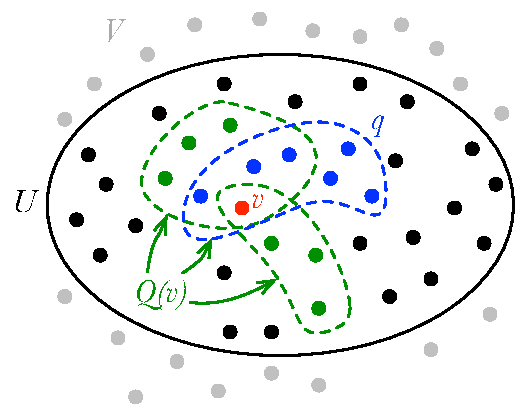
\includegraphics[width=8 cm]{Figures/vqQUV}
\caption{\bf \small The five levels of a Stellar network or FBAS}
\label{fig:vqQUV}
\end{figure}

Using the usual notation $2^X$ for the power set\footnote{The power set of a set $X$ is the set of all possible subsets of $X$ \cite{Cameron2008}. For a set of $N$ elements, its power set turns out to have $2^N$ elements, hence the notation.} of the set $X$, $2^V$ is the power set of $V$, i.e.\ the set of all possible quorum slices. At the next level, $2^{2^V}$ is the power set of quorum slices, i.e. the set of all possible \emph{sets} of quorum slices. Figure \ref{fig:SliceAndQ} shows a visualization of the elements of these kinds of power sets.

\begin{figure}[h]
\centering
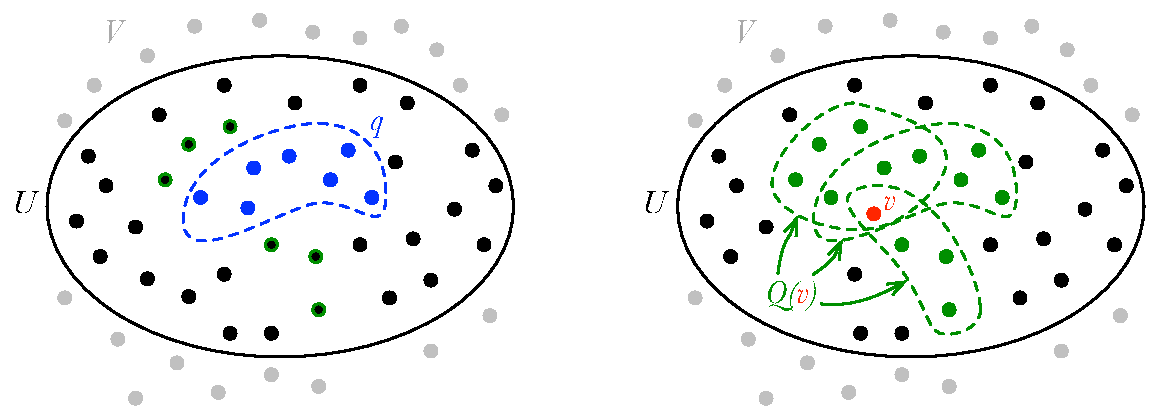
\includegraphics[width=15 cm]{Figures/SliceAndQ}
\caption{\bf \small LEFT: a) $q$ is an element of $2^V$. RIGHT: b) $Q(v)$ is an element of $2^{2^V}$.}
\label{fig:SliceAndQ}
\end{figure}

The function $Q$ assigns to each node $v \in V$ a set of slices $\{ q_1, q_2, \cdots, q_k \}$. Here the curly brackets denote set and $k$ is the number of slices for a given node $v$. Formally,
\begin{align}
Q\colon V \rightarrow 2^{2^V} \setminus \emptyset,
\end{align}
where $\setminus \emptyset$ means that the empty set is not in the range of this function ($Q(v)$ can never be empty).\footnote{It is not immediately clear whether this is a consequence of how this function operates or whether it is a requirement that we are adding arbitrarily to ensure that it does what we need. \textcolor{red}{TBD.}} In general,
\begin{align}
\forall v \in V, \forall q \in Q(v), \qquad v \in q,
\end{align}
which reads `For all nodes $v$ members of the set $V$ and for all slices $q$ members of the set $Q(v)$, node $v$ is a member of some slice $q$'.
\begin{defin}
A Federated Byzantine Agreement System \emph{(\textbf{FBAS})} is a pair $(V, Q)$.
\end{defin}
\begin{defin}
A set of nodes $U \subseteq V$ in a FBAS $(V, Q)$ is a \emph{\textbf{quorum}} iff $U \ne \emptyset$ and $U$ contains a slice for each member:
\begin{align}
\forall v \in U, \exists q \in Q(v) \ | \  q \subseteq U.
\end{align}
\end{defin}
In English: for all $v$ members of a quorum $U$, there exists a slice $q$, member of $Q(v)$, such that the slice is a subset of, or equal to, the quorum $U$. A quorum can also be described as a set of nodes sufficient to reach agreement.
\begin{defin}
A \emph{\textbf{quorum slice}} $q$ is a subset of a quorum $U$ sufficient to convince a particular node $v$ of agreement.
\end{defin}
Therefore, a quorum slice is usually smaller than a quorum, as shown in the figures above. The `convincing' is depicted graphically by an arrow that indicates dependence between nodes in a manner analogous to inheritance in UML class diagrams. For example, as shown in Figure \ref{fig:convincing}a, $v_2$ can convince $v_1$ but not vice versa, i.e.\ $v_1$ depends on itself and on $v_2$ while $v_2$ depends only on itself. Figure \ref{fig:convincing}b shows the corresponding slices. Note that in this simple case the quorum of this set of nodes $V = \{ v_1, v_2 \}$ equals the slice for $v_1$: $V = U = q(v_1) = \{ v_1, v_2 \}$, whereas the set of slices $Q(v_1)$ is written $Q(v_1) = \{ \{ v_1, v_2 \} \}$, where the outer curly brackets indicate the set of slices $Q(v_1)$ and the inner curly brackets indicate the slice $q_1 = q(v_1)$.

\begin{figure}[h]
\centering
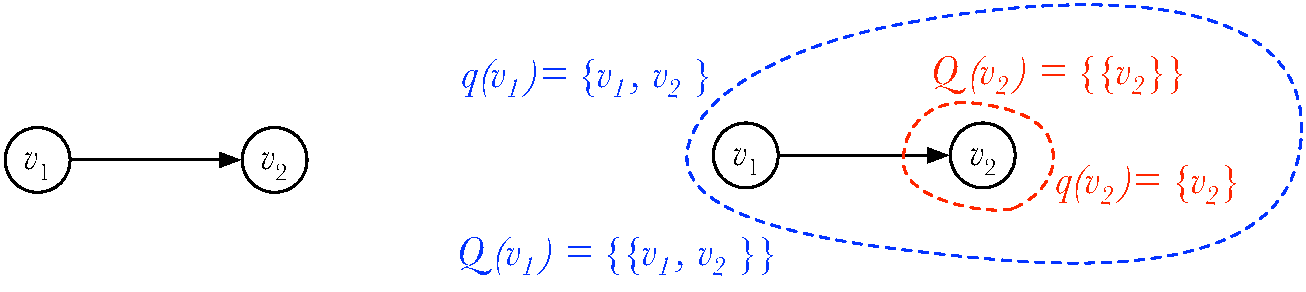
\includegraphics[width=15 cm]{Figures/convincing}
\caption{\bf \small LEFT: a) $v_2$ can convince $v_1$ but not vice versa. RIGHT: b) The slices of $v_1$ and of $v_2$.}
\label{fig:convincing}
\end{figure}

Figure \ref{fig:example1} shows a more complex interdependence between a set of 4 nodes. The arrows imply that $v_2$, $v_3$, and $v_4$ each has the same slice, e.g.\ $Q(v_2) = \{\{ v_2, v_3, v_4 \} \}$. In this example, although $\{\{ v_2, v_3, v_4 \} \}$ is a quorum, the smallest quorum involving $v_1$ must involve all four nodes.

\begin{figure}[h]
\centering
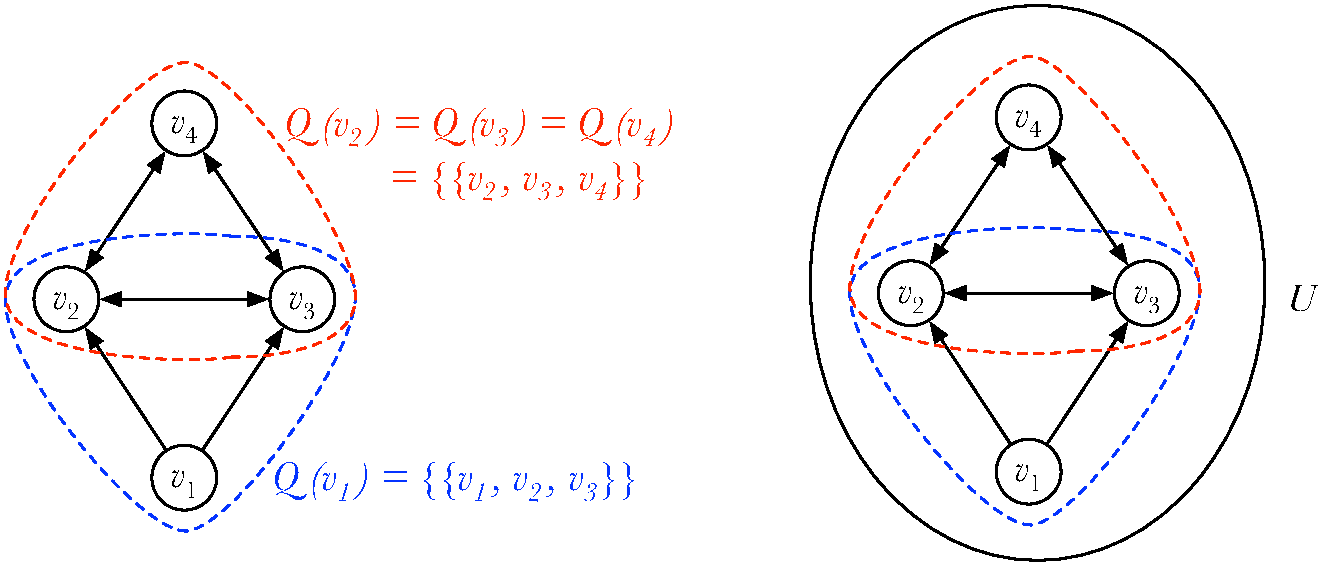
\includegraphics[width=15 cm]{Figures/example1}
\caption{\bf \small LEFT: a) The slices of this network. RIGHT: b) The smallest quorum involving $v_1$. (After \cite{Mazieres2016})}
\label{fig:example1}
\end{figure}

In traditional, non-federated Byzantine systems all nodes have the same slices. Therefore, non-federated systems do not distinguish between slices and quorums:
\begin{align}
\forall v_i, v_j \in V, \qquad Q(v_i) = Q(v_j). \qquad\qquad \text{[BAS]} 
\end{align}
In our case, instead, in general we have that
\begin{align}
\forall v_i, v_j \in V, \qquad Q(v_i) \ne Q(v_j). \qquad\qquad \text{[FBAS]} 
\end{align}
The important point made by Mazi\`eres is that whereas BAS is not scalable, as exemplified by the huge CPU overhead the Bitcoin consensus protocol requires, FBAS is scalable.

\begin{center}
\small
\frame{\colorbox{light-gray}{\makebox[16.5cm]{\parbox{16.5cm}{
\vspace{.2cm}
\begin{quote}
\textbf{Example 2}

It is worth discussing a second example from Mazi\`eres, as shown in Figure \ref{fig:example2}. The figure shows three new notational concepts: a reflexive dependence arrow can be drawn explicitly, sets of nodes can be grouped explicitly into separate tiers, and the dependence arrows can carry specific labels. For example, the label on the reflexive arrow on the top tier indicates that at least 3 nodes are needed for consensus. According to the definitions above for the arrow directions, the top tier does not depend on the tiers below, and it is precisely for this reason that it is the `top' tier.
\end{quote}
\vspace{-.6cm}
\begin{figure}[H]
\centering
\captionsetup{width=11cm}
\frame{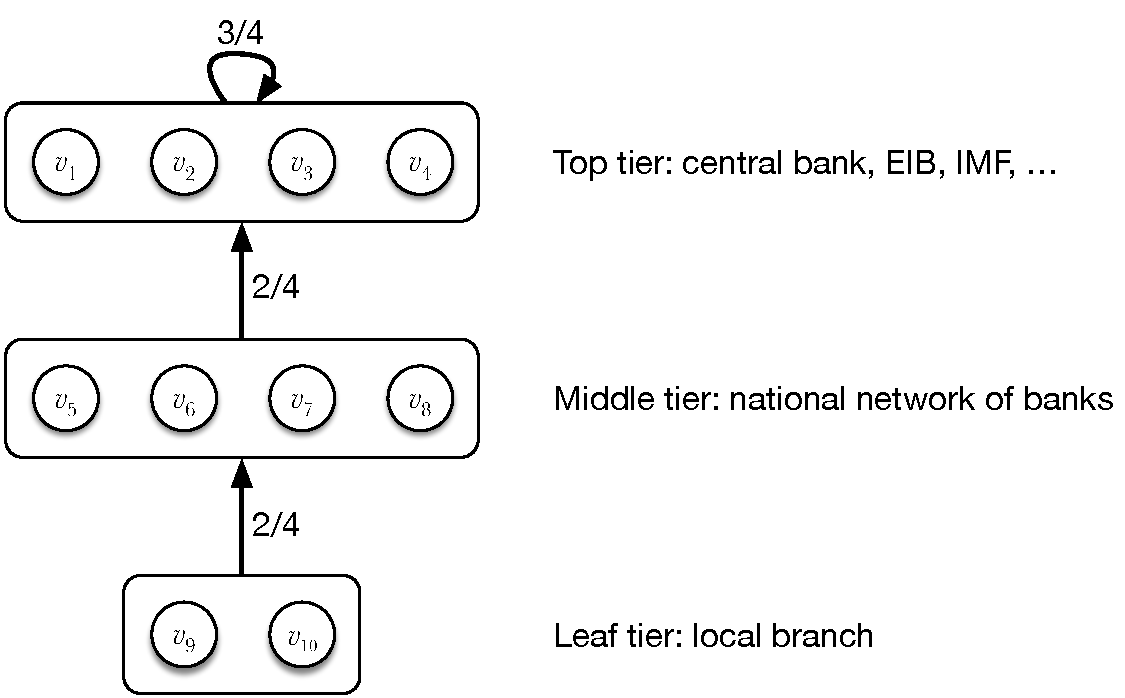
\includegraphics[width=11 cm]{Figures/example2}}
\caption{\bf \small Three-tier network with possible mapping to INTERLACE circuit architecture. (After \cite{Mazieres2016})}
\label{fig:example2}
\end{figure}
\begin{quote}
\vspace{-.5cm}
The arrow between the middle and top tiers indicates that the slice of any one node from the middle tier is composed of itself plus any two of the tier above. The slice of the either $v_9$ or $v_{10}$ is composed of itself plus any two nodes from the middle tier. Since each of these, in turn, depends on any two of the nodes of the top tier, the size of the slice will be at least 5 and at most 7 nodes. In this figure, the top tier according to Mazi\`eres could be composed by a number of global financial institutions, whereas in the INTERLACE case it would be only the single Sardex S.p.A.\ company. However, we retained the example as presented by Mazi\`eres in order to continue to develop and explain the dependencies between nodes and sets of nodes.
\end{quote}

\vspace{.2cm}
}}}}
\end{center}














